\documentclass[a4j,uplatex,dvipdfmx]{jsarticle}
\usepackage{amsmath}
\usepackage{tcolorbox}
\tcbuselibrary{breakable, skins, theorems}

\title{確率情報理論第hoge回 解答}
\author{加藤まる}
\date{2020/03/01}

\begin{document}
\maketitle
\bf キーワード:
\rm

\section*{本日の問題解答}
集合$A=\{ 1,2\}$と$B=\{ 1,2,3 \}$に対して、次の表に示す同時確率にしたがい$A \times B$の要素をとる確率変数(X,Y)を考える。
\begin{itemize}
  \item[(1)]エントロピーH(X)とH(Y)を求めよ。
  XとYの周辺確率をそれぞれ$P_X$と$P_Y$とすれば、$P_X(1)=1/2,~P_X(2)~1/2,~P_Y(1)=1/4,~P_Y(2),~P_Y(3)=1/4$となる。
  したがって、
  \begin{equation}
    H(X)=-\frac{1}{2}\log{\frac{1}{2}}-\frac{1}{2}\log{\frac{1}{2}}=1
  \end{equation} 
  \begin{equation}
    H(Y)=-\frac{1}{4}\log{\frac{1}{4}}-\frac{1}{2}\log{\frac{1}{2}}-\frac{1}{4}\log{\frac{1}{4}}=1.5
  \end{equation} 
  \item[(2)]同時エントロピーH(X,Y)を求めよ。
  \begin{equation}
    H(X,Y)=-4\times \frac{1}{8}\log{\frac{1}{8}}-2\times \frac{1}{4}\log{\frac{1}{4}}=2.5
  \end{equation} 
  \item[(3)]条件付きエントロピー$H(X|Y)$と$H(Y|X)$を求めよ。
  条件付き確率$P_{X|Y}$は
  \begin{equation}
    P_{X|Y}(1|1)=\frac{1}{2},~~P_{X|Y}(2|1)=\frac{1}{2},~~P_{X|Y}(1|2)=\frac{1}{2}
  \end{equation} 
  \begin{equation}
    P_{X|Y}(2|2)=\frac{1}{2},~~P_{X|Y}(1|3)=\frac{1}{2},~~P_{X|Y}(2|3)=\frac{1}{2}
  \end{equation}
  となる。したがって、
  \begin{equation}
    \begin{split}
      H(X|Y)&=\frac{1}{4}H(X|Y=1)+\frac{1}{2}H(X|Y=2)+\frac{1}{4}H(X|Y=3)\\
      &=\frac{1}{4}\left( -\frac{1}{2}\log{\frac{1}{2}}-\frac{1}{2}\log{\frac{1}{2}} \right)+\frac{1}{2}\left( -\frac{1}{2}\log{\frac{1}{2}}-\frac{1}{2}\log{\frac{1}{2}} \right)+\frac{1}{4}\left( -\frac{1}{2}\log{\frac{1}{2}}-\frac{1}{2}\log{\frac{1}{2}} \right)\\
      &=1
    \end{split}
  \end{equation}
  また、条件付き確率$P_{Y|X}$は
  \begin{equation}
    P_{Y|X}(1|1)=\frac{1}{4},~~P_{Y|X}(2|1)=\frac{1}{2},~~P_{Y|X}(3|1)=\frac{1}{4}
  \end{equation}
  \begin{equation}
    P_{Y|X}(1|2)=\frac{1}{4},~~P_{Y|X}(2|2)=\frac{1}{2},~~P_{Y|X}(3|2)=\frac{1}{4}
  \end{equation}
  となる。したがって、
  \begin{equation}
    \begin{split}
      H(Y|X)&=\frac{1}{2}H(Y|X=1)+\frac{1}{2}H(Y|X=2)\\
      &=\frac{1}{2}\left( -\frac{1}{4}\log{\frac{1}{4}}-\frac{1}{2}\log{\frac{1}{2}}-\frac{1}{4}\log{\frac{1}{4}} \right)+\frac{1}{2}\left( -\frac{1}{4}\log{\frac{1}{4}}-\frac{1}{2}\log{\frac{1}{2}}-\frac{1}{4}\log{\frac{1}{4}} \right)\\
      &=1.5
    \end{split}
  \end{equation}
  \item[(4)]相互情報量I(X;Y)を求めよ。
  $P_{XY}$ならびに$P_X$と$P_Y$を用いれば、
  \begin{equation}
    \begin{split}
      I(X;Y)&=\frac{1}{8}\log{\frac{\frac{1}{8}}{\frac{1}{2}\times \frac{1}{4}}}+\frac{1}{8}\log{\frac{\frac{1}{8}}{\frac{1}{2}\times \frac{1}{4}}}+\frac{1}{4}\log{\frac{\frac{1}{4}}{\frac{1}{2}\times \frac{1}{2}}}+\frac{1}{4}\log{\frac{\frac{1}{4}}{\frac{1}{2}\times \frac{1}{2}}} \\
      &+\frac{1}{8}\log{\frac{\frac{1}{8}}{\frac{1}{2}\times \frac{1}{4}}}+\frac{1}{8}\log{\frac{\frac{1}{8}}{\frac{1}{2}\times \frac{1}{4}}}\\
      &=0
    \end{split}
  \end{equation}
\end{itemize}
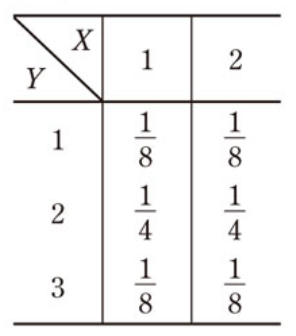
\includegraphics[width=5cm]{sec19fig.png}


\end{document}